\chapter{Testing}

\section{Original Data}

Here we will explore the results of different classifiers and active learning strategies on the original data. The original data consisted of data shown previously in Figure \ref{fig:original_english_counts} and discretely in Table \ref{tab:en_data_counts} in Appendix \ref{app:attachments}. 

\subsection{Active Learning with PWC and RBF Kernel}

In Figure \ref{fig:plot_all_results_rbf} we have the train and test errors for four different active learning sampling strategies and we can see that xPAL and PAL both perform relatively well before starting to over-fit the training data. We reviewed the resulting error data and xPAL outperformed PAL by about 1.5\%. However, xPAL has much faster running time compared to PAL.

We weren't satisfied with the testing error which leveled out to about 70\% for each sampling strategy. PAL and xPAL were able to rapidly reduce the testing error early on in the training process while random selection and QBC weren't able to determine the data with the highest information gain. 

\begin{figure}[ht]
  \centering
  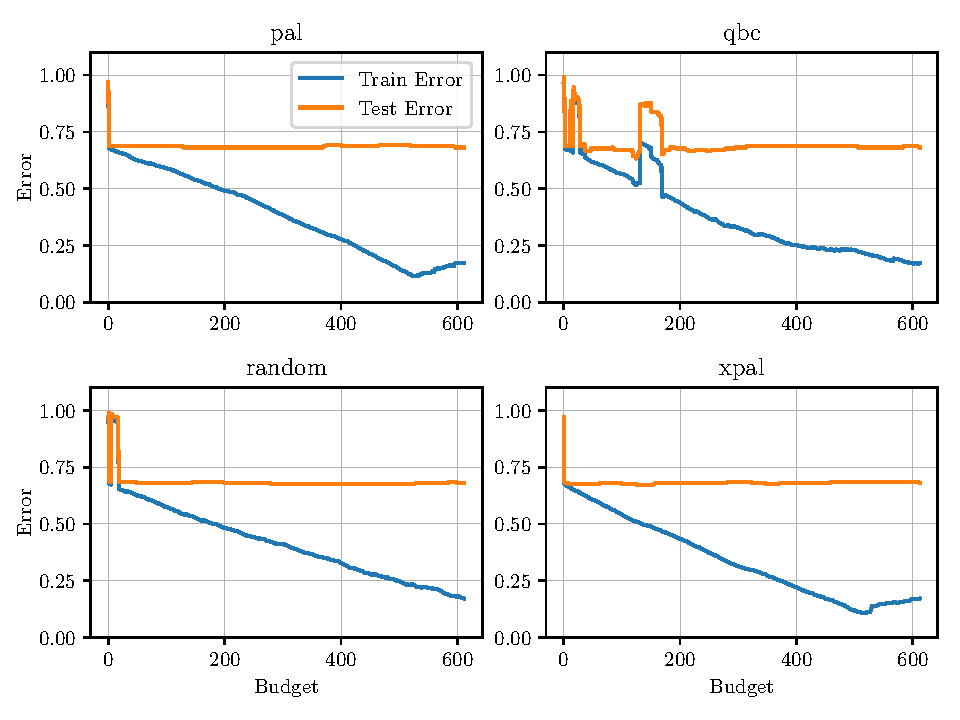
\includegraphics[width=\textwidth]{../img/plot_all_results_rbf.pdf}
  \caption{Train and test error using different query strategies and RBF kernel for the PWC classifier.}
  \label{fig:plot_all_results_rbf}
\end{figure}

The radial bias function (RBF) kernel is a popular kernel function. It is defined as:

\begin{equation}
    K(x_i, x_j) = \exp\left(- \frac{\left\| x_i - x_j \right\|^2}{2 \sigma^2}\right)
\label{eq:rbf_kernel}
\end{equation}

where $\sigma$ is a parameter that controls the smoothness of the kernel and $x_i$ and $x_j$ are the two points in the feature space to compare. As seen in the Figure \ref{fig:plot_all_results_rbf} when the PWC classifier uses the RBF kernel it doesn't perform well with this data.

\subsection{Active Learning with PWC and Cosine Kernel}

In Figure \ref{fig:plot_all_results_cosine} we have the train and test errors for the same four different active learning sampling strategies tested on the same data. The only change was that we used Cosine kernel instead of the RBF kernel.The Cosine kernel is another important kernel function that is used in many machine learning algorithms. It is defined as:

\begin{equation}
    K(x_i, x_j) = \frac{x_i \cdot x_j}{\left\| x_i \right\| \left\| x_j \right\|}
\label{eq:cosine_kernel}
\end{equation}

where $x_i$ and $x_j$ are the two points in the feature space to compare. We found that using the Cosine kernel reduced the test error across the board by $\sim$15\%.  

\begin{figure}[ht]
  \centering
  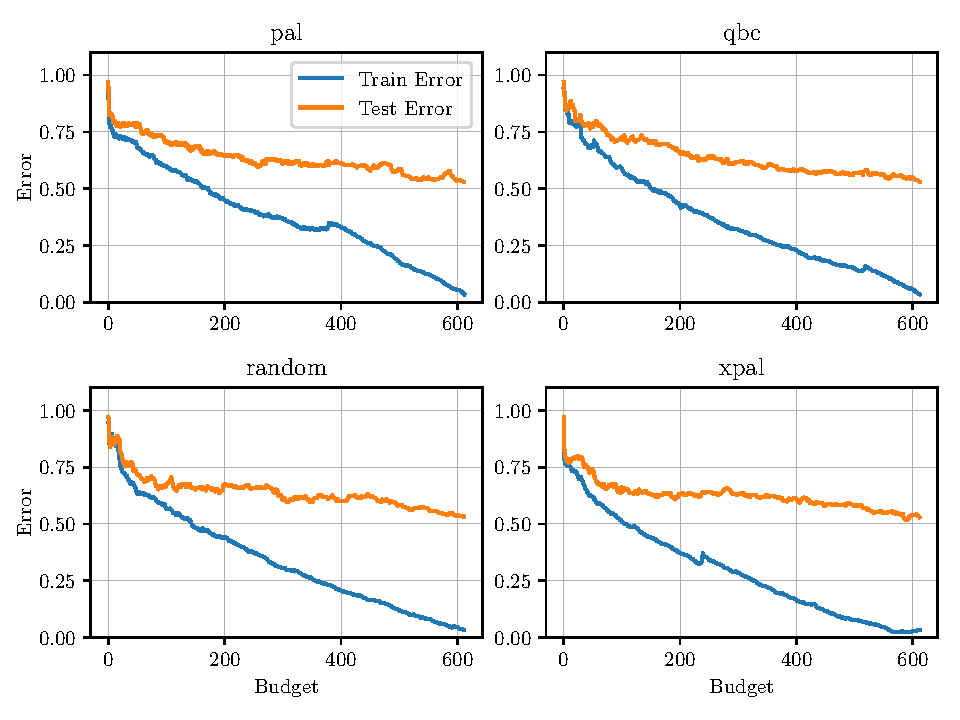
\includegraphics[width=\textwidth]{../img/plot_all_results_cosine.pdf}
  \caption{Train and test error using different query strategies and Cosine kernel for the PWC classifier.}
  \label{fig:plot_all_results_cosine}
\end{figure}


In Figure \ref{fig:plot_all_results_cosine} PAL and xPAL were able to reduce the training error, by about 20\% and 25\% respectively, early in the training process compared to random selection and QBC. We also tested the other sampling strategies with the Cosine kernel and found that the results were similar. The other sampling strategies and their test data results are shown in Table \ref{fig:cos_test_results} along with the test data from Figure \ref{fig:plot_all_results_cosine}. 


\begin{figure}[ht]
    \centering
    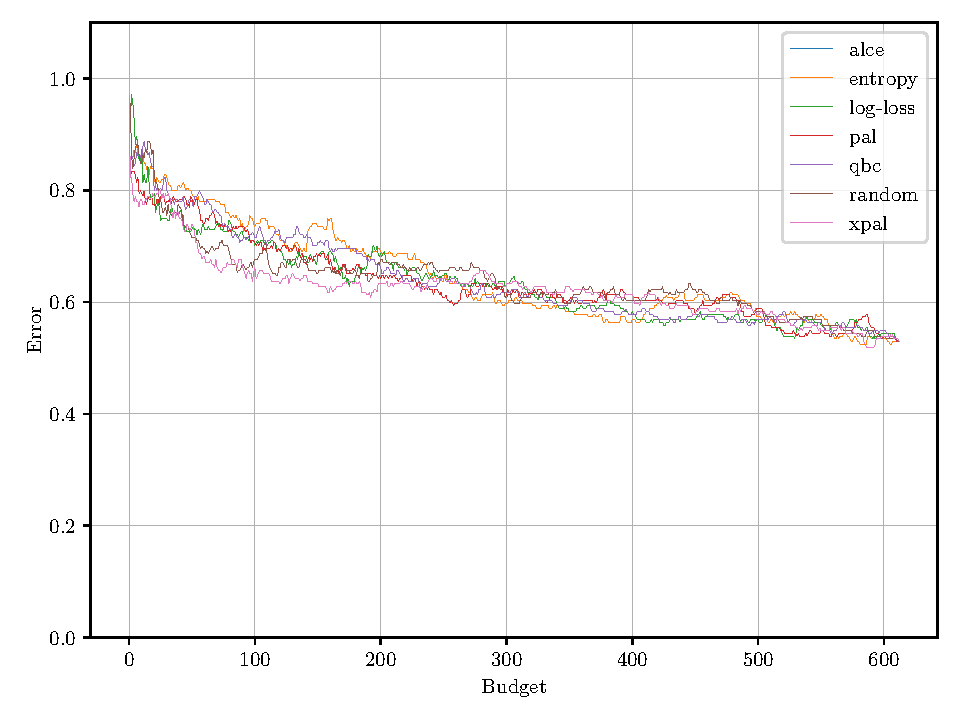
\includegraphics[width=\textwidth]{../img/plot_kernel_cos_test_results.pdf}
    \caption{Comparing test error using different query strategies and Cosine kernel for the PWC classifier.}
    \label{fig:cos_test_results}
\end{figure}

We can see that the sampling strategies test performance converges over time (as we are using the same data and classifier) but xPAL has the appears to have an absolute minimum near the 600 budget mark in comparison to all sampling strategies. XPAL also appears to be performing well early on in the training process, in the 100-200 budget range.

Figure \ref{fig:cos_test_results} shows that xPAL seems to be performing the best with our data but we wanted to see if we ran more tests with different train-test splits how the results would average out and which sampling strategy would perform the best. We ran 10 different data splits with each of the 7 sampling strategies and then took the average to get a smoother curve compared to the single run results shown in Figure \ref*{fig:cos_test_results}. The results for this experiment are shown in Figure \ref{fig:cos_avg_test_results}.

\begin{figure}[ht]
    \centering
    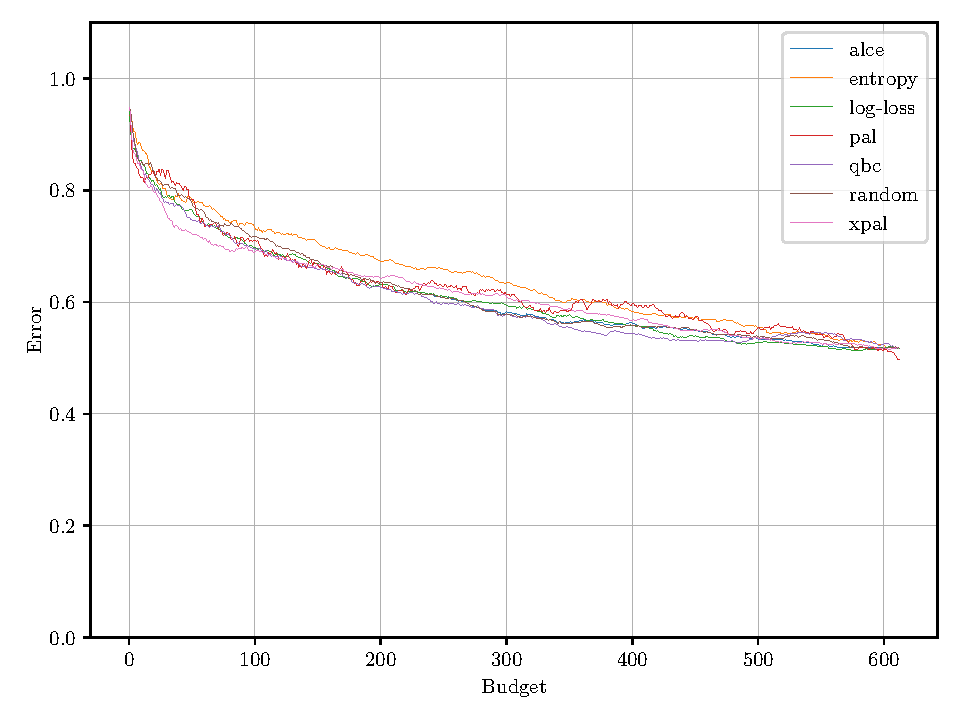
\includegraphics[width=\textwidth]{../img/plot_kernel_cos_averaged_test_results.pdf}
    \caption{Comparing test error using different query strategies and Cosine kernel for the PWC classifier with results averaged over 10 different data splits.}
    \label{fig:cos_avg_test_results}
\end{figure}


\subsection{Scikit-Learn Classifier Evaluation}

We also decided to try out the boilerplate classifiers from Scikit-Learn to compare performances. Again we used the original data with the same TF-IDF vectorizer as used with the previous active learning models to stay consistent. Cross validation was also used here but was not used in the previous sections. We decided to use the Cosine kernel when using LinearSVC as we learned that the performance increased in comparison to the RBF kernel when using PWC. 

The results for a variety of different classifiers are shown in Figure \ref{fig:explore_classifiers}. In the box-plot, the whiskers extend from the box to the furthest data points that are within 1.5 times the inter-quartile range (IQR) of the box. Any data points that are beyond the whiskers are considered outliers and are plotted as individual points or symbols (diamonds) as seen in Figure \ref{fig:explore_classifiers}.

\begin{figure}[ht]
  \centering
  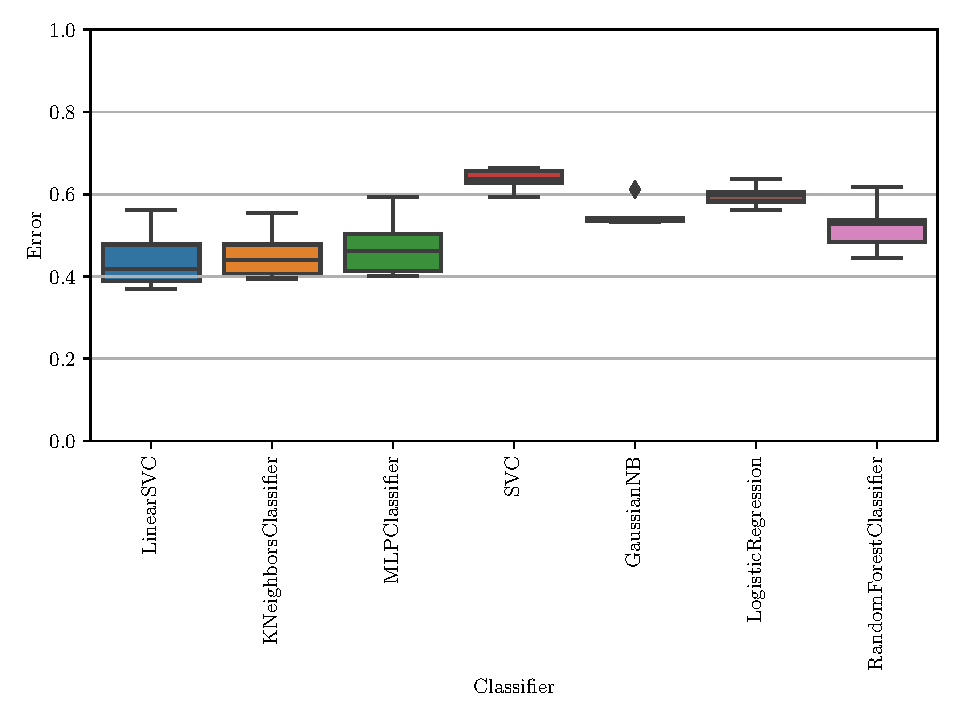
\includegraphics[width=\textwidth]{../img/plot_explore_classifiers.pdf}
  \caption{Performance of standard Scikit-Learn classifiers without optimization.}
  \label{fig:explore_classifiers}
\end{figure}

The LinearSVC classifier performed best compared to other classifiers and it is a fast running algorithm even with data that has a large feature set. We decided to look further into LinearSVC and create a few models to evaluate its performance. We created three models, the first was a boilerplate LinearSVC with no argument modifications, the second model used the class weights parameter set to 'balanced'. The 'balanced' mode uses the values of y to automatically adjust weights inversely proportional to class frequencies in the input data as $n\_samples / (n\_classes * np.bincount(y))$. 

For the third test we created a dictionary of weights for each class using the Cosine decay function. The weights for each category ranged from 0.1 to 1.0 where the most frequent classes had smaller weights. The results are shown in Table \ref{tab:lsvc_errors}. The Cosine decay function is defined as:

\begin{equation}
    w_i = \frac{1}{2} \left(1 + \cos \left(\frac{\pi t}{T}\right)\right)
\label{eq:cosine_decay}
\end{equation}

where $w_i$ is the weight for the $i^{th}$ class, $t$ is the current iteration, and $T$ is the total number of iterations. The Cosine decay function is a common function used for weights in machine learning algorithms.


\begin{table}[!ht]
\centering
\caption{Error for three differing LinearSVC models.}
\begin{tabular}{lr}
\toprule
               Model &  Error \\
\midrule
Cosine Decay Weights &  0.392 \\
         Boilerplate &  0.407 \\
    Balanced Weights &  0.441 \\
\bottomrule
\end{tabular}

\label{tab:lsvc_errors}
\end{table}

We also tested some other models that we expected to perform well, namely K-Nearest Neighbors and Neural Networks. The results are shown in Table \ref{tab:best_errors}. We can see that the K-Nearest Neighbors classifier and the Tensor Flow Neural Network classifier performed slightly worse compared to LinearSVC.

\begin{table}[!ht]
\centering
\caption{Keywords from TF-IDF with Chi Squared using the original data.}
\begin{tabular}{lr}
\toprule
         Model &  Error \\
\midrule
     LinearSVC &  0.392 \\
Neural Network &  0.446 \\
           KNN &  0.451 \\
\bottomrule
\end{tabular}

\label{tab:best_errors}
\end{table}

We attempted to boost performance from the LinearSVC classifier using GridSearchCV and Bagging but were not able to make significant improvements in performance from what we observed in Table \ref{tab:best_errors}. The precision-recall curve is shown in Figure \ref{fig:pr_curve} and the confusion matrix is shown in Figure \ref{fig:confusion_matrix} for the best performing LinearSVC classifier.

\begin{figure}[ht]
  \centering
  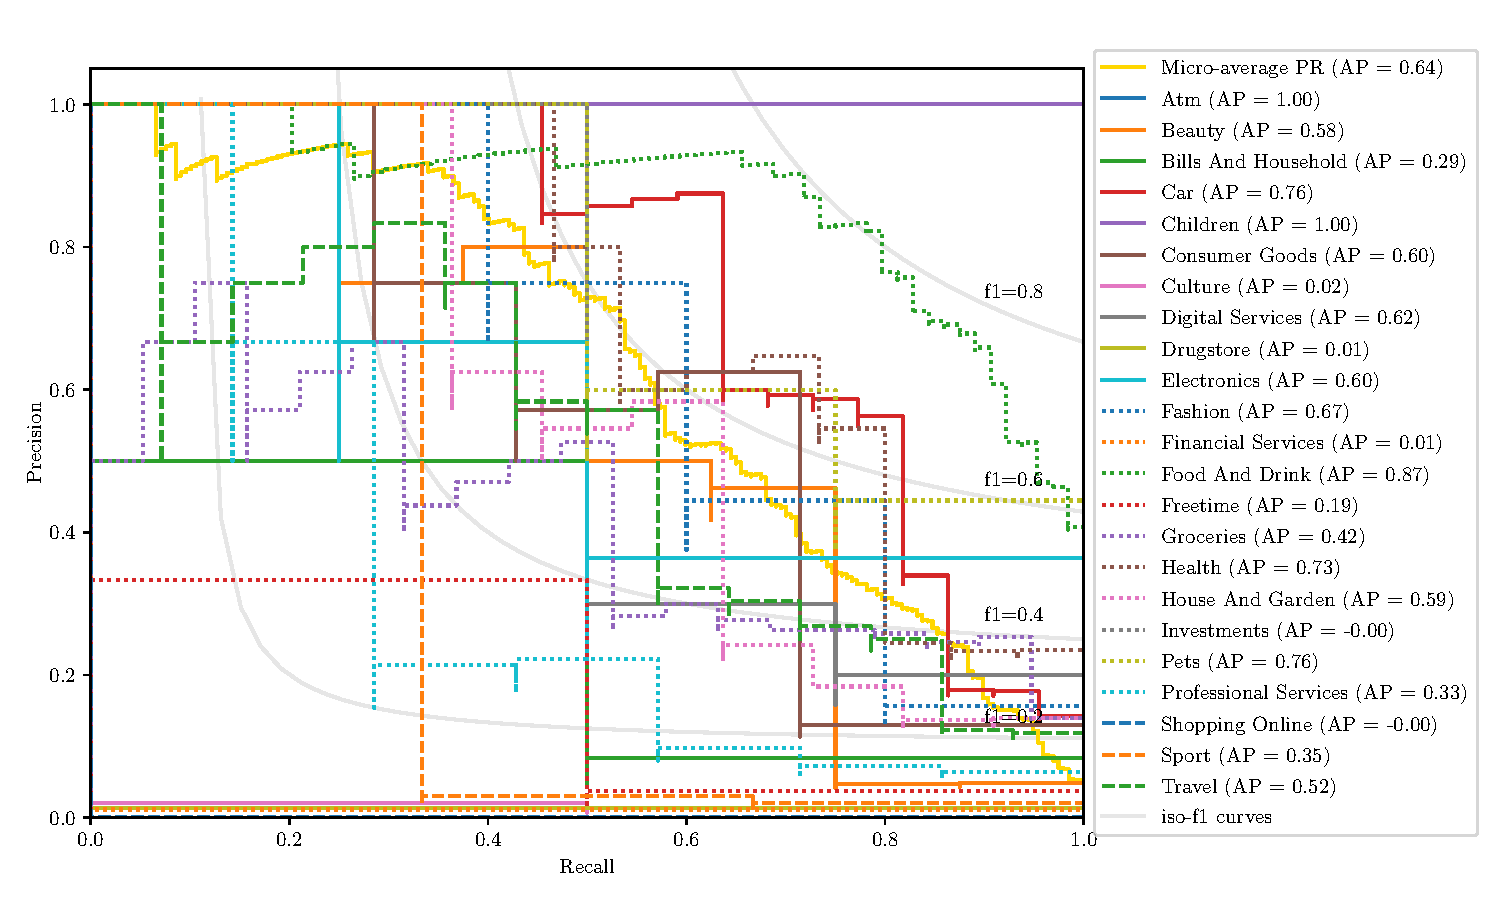
\includegraphics[width=\textwidth]{../img/plot_pr_curve.pdf}
  \caption{Precision-recall curve for the best performing LinearSVC classifier.}
  \label{fig:pr_curve}
\end{figure}

It is important to note that the precision-recall curve is not a perfect metric for this problem as the classes are not balanced. We can see this imbalance clearly in Figure \ref{fig:pr_curve} where we have straight lines and large clear steps in some plotted category lines. This is a result of having a small number of data in a class. However, we can also see that for some classes the precision is very high even though we have very few data points. Here we are namely concerned with the 'Culture' and 'Beauty' categories which have 10 and 31 data points respectively. The confusion matrix shown in Figure \ref{fig:confusion_matrix} may be a better metric for visualizing this data. 

\begin{figure}[ht]
  \centering
  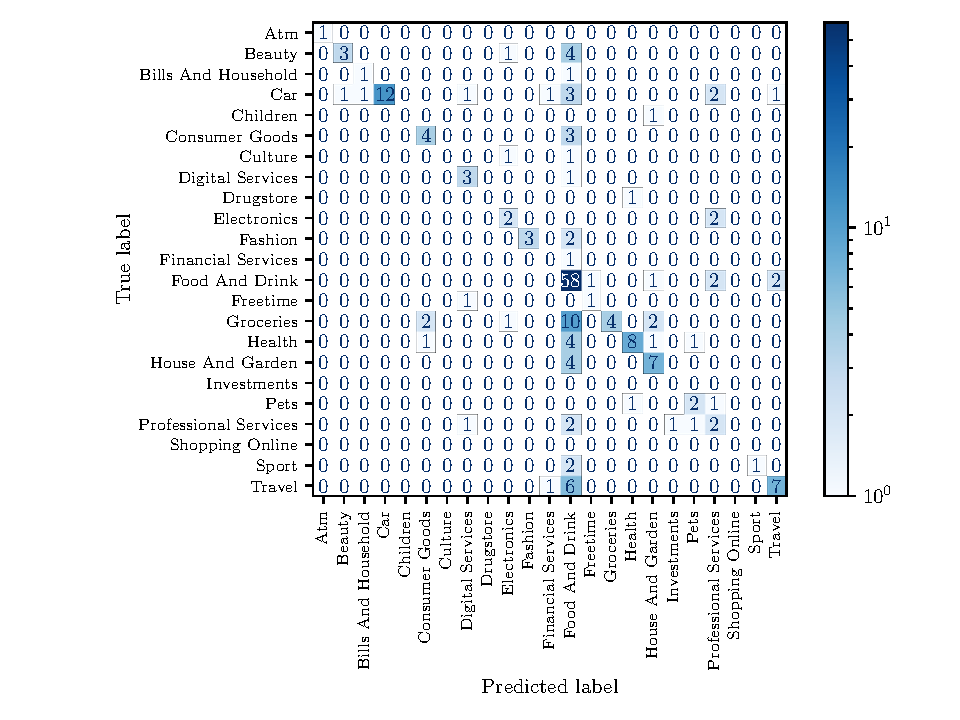
\includegraphics[width=\textwidth]{../img/plot_cm_LinearSVC.pdf}
  \caption{Confusion matrix for the best performing LinearSVC classifier.}
  \label{fig:confusion_matrix}
\end{figure}


\section{Original and Additional Data}

In this section we will explore the results of different classifiers and active learning strategies on the original data plus the additional data.